\chapter{Das REST Architekturkonzept}
\section{Entstehung}
Das Architekturkonzept des Representational State Transfer wurde erstmals im Jahr 2000 von Roy T. Fielding erwähnt, definiert und mit dem Akronym REST bezeichnet.\cite[76]{REST}
Es enthält eine Reihe von Prinzipien für die Entwicklung von verteilten Systemen im Web mit besonderem Fokus auf den Schnittstellen zwischen den einzelnen Komponenten.
Dabei baut REST auf der Client-Server-Architektur auf und hatte durch die Arbeit vib Fielding in den HTTP- und URI-Arbeitsgruppen direkten Einfluss auf die Entwicklung von der beiden Standards, wodurch jene Schnittstellen im Web definiert werden.\cite[vgl.][4,105f.]{REST}
REST beschreibt größtenteils die Architektur des Web selbst und ist daher nicht auf APIs ausgelegt oder beschränkt.

\section{Grundlagen}
\subsubsection{Ziele von REST}
Die Ziele und Vorteile der REST Architektur lassen sich folgendermaßen zusammenfassen:
\foreignblockcquote{english}[105]{REST}{REST provides a set of architectural constraints that, when applied as a whole, emphasizes scalability of component interactions, generality of interfaces, independent deployment of components, and intermediary components to reduce interaction latency, enforce security, and encapsulate  legacy  systems.}
Diese Ziele werden erreicht durch eine Reihe von Anforderungen.
\subsubsection{Komponenten und Prinzipien}
Die REST Architektur baut auf der weit verbreiteten Client-Server Architektur auf und definiert den Begriff der Ressource als Abstraktion für jede Art von Information, die Ziel einer Client-Anfrage ist.\cite[vgl.][88f.]{REST}
Als Beispiele für Ressourcen nennt Fielding selbst: \textcquote[88]{REST}{a document or image, a temporal service [\dots], a collection of other resources, a non-virtual object (e.g.\ a person).}
Eine Ressource wird durch einen Bezeichner bekannt gemacht und ist damit für einen Client abrufbar.
Der Bezeichner bleibt gleich, selbst wenn sich die damit identifizierte Ressource ändert.
Die Kommunikation einer Ressource vom Server zum Client erfolgt über eine Repräsentation der Ressource, d.h.\ ein Datenformat, welches vom Server festgelegt, oder durch Content-Negotiation zwischen Client und Server ausgehandelt wird.
Somit bleibt der Ursprung der Daten hinter der Serverschnittstelle versteckt.
Die Antwort des Servers enthält die Daten der Repräsentation und deren Metadaten.
Anfrage und Antwort enthalten außerdem Kontrolldaten, \zB{} HTTP Request Methods, Status Codes und Header, um die Bedeutung der Nachricht zu vermitteln.\cite[vgl.][90f.]{REST}
\begin{table}[h!]
  \begin{center}
    \caption{REST Data Elements}\label{tab:REST Data Elemens}
    \begin{tabularx}{\textwidth}{XXX}
      \toprule
      \textbf{Data Element} & \textbf{Web Equivalent} & \textbf{Example}\\
      \midrule
      resource & the intended conceptual target of a hypertext reference & a list of events\\
      resource identifier & URI & http://example.com/events\\
      representation data & HTML, JSON Document, PNG image & \{events:[\{title:\dots\},\{\dots\}]\}\\
      representation metadata & media type, last-modified time, ETag & Content-Type: application/json\\
      & & Content-Encoding: gzip\\
      control data & if-modified-since, cache-control, request method & GET, Cache-Control: no-cache\\
    \end{tabularx}
  \end{center}
\end{table}
\par
REST ist zustandslos, sodass jede Anfrage vom Client zum Server alle für deren Verarbeitung notwendigen Informationen beinhalten muss.
Ein Client speichert gewöhnlich seinen Zustand, während auf Serverseite keine Zustandsinformationen über mehrere Anfragen hinweg gespeichert werden, wie es zum Beispiel bei Sessions der Fall ist.
Aufgrund dieser Eigenschaft wird im Zusammenhang mit REST auch von einer \foreigntextcquote{english}[83]{REST}{Client-Cache-Stateless-Server[-Architektur]} gesprochen.
Hieraus ergeben sich drei Vorteile:\cite[vgl.][79]{REST}
\begin{itemize}
  \item Sichtbarkeit:
  Jede Anfrage kann separat untersucht und gecacht werden, ohne weitere Informationen zu benötigen.
  \item Zuverlässigkeit:
  Anfragen können atomar betrachtet und bei Teilfehlern kann ein stabiler Systemzustand leicht wiederhergestellt werden.
  \item Skalierbarkeit:
  Da ein Server Zustandsinformationen nur für die Dauer der Verarbeitung einer Anfrage speichert, können Ressourcen schnell wieder freigegeben werden.
\end{itemize}
Nachteil dieser Anforderung ist eine verringerte Netzwerkperformance, da bei sequenziellen Anfragen an einen Server, Daten zur Clientidentifikation, Authentifizierung oder aus vorangegangene Antworten erneut gesendet werden müssen.
Die verringerte Kopplung führt ebenfalls dazu, dass die Kontrolle des Servers über das Verhalten der Clientanwendung reduziert wird.
\par
Clientseitiges Speichern von erhaltenen Daten (Caching) erlaubt die Wiederverwendung früherer Serverantworten für zukünftige, gleiche Anfragen und ist sinnvoll, da die gefühlte Performance durch Verringerung der durchschnittlichen Latenz erhöht wird.
Dadurch wird die Effizienz und Skalierbarkeit der Anwendung erhöht, obwohl die Latenz jeder einzelnen Anfrage durch den Cache-Lookup erhöht wird.
Je mehr die gespeicherten Daten von den tatsächlichen Daten abweichen, desto mehr verringert sich die Verlässlichkeit derselben.\cite[vgl.][80]{REST}
GET-Requests werden von Webbrowsern implizit gecacht, wobei Server das gewünschte Caching-Verhalten explizit erlauben und verbieten können.

REST beschreibt drei Typen von Komponenten:\cite[vgl.][96]{REST}
\begin{itemize}
  \item User Agent:
  Dies kann ein Webbrowser bzw.\ die Benutzeranwendung sein, in jedem Fall jedoch der letztendliche Empfänger der Antwort.
  \item Origin Server:
  Die endgültige Quelle der Repräsentation einer Ressource und der letztendliche Empfänger von Request, die zu Modifikationen der Daten führen.
  \item Intermediary (Zwischenkomponenten):
  Diese befinden sich zwischen User Agent und Origin Server und können sowohl als Client, als auch als Server agieren. Sie leiten Anfragen und Antworten weiter, können diese aber auch modifizieren. Je nach Anwendungsfall spricht man hier von einem Gateway oder Proxy.
\end{itemize}
Für die Schnittstellen der Komponenten gelten folgende Grundsätze:\cite[vgl.][82]{REST}
\begin{itemize}
  \item Ressourcen müssen durch einen Bezeichner eindeutig identifizierbar sein.
  \item Die Interaktion mit einer Ressource, d.h.\ das Abfragen und Manipulieren derselben erfolgt über eine Repräsentation der Ressource.
  \item Nachrichten müssen so selbsterklärend sein, dass sie von der Schnittstelle verstanden und verarbeitet werden können.
  \item \foreigntextcquote{english}[82]{REST}{hypermedia as the engine of application state} (HATEOAS): Der Hypertext beschreibt den Zustand der Anwendung und die Möglichkeiten der Veränderung desselben.
\end{itemize}
\par
Durch die generischen Client- und Serverschnittstellen, die selbstbeschreibenden Nachrichten und die zustandslose Kommunikation kann eine REST Anwendung leicht von Schichten profitieren.
Keine einzelne Komponente benötigt Kenntnis des gesamten Informationsweges, sondern sieht nur die Komponenten, mit denen sie direkt interagiert, sodass zwischen
User-Agent und Origin-Server Zwischenkomponenten eingeführt werden können, um spezifische Aufgaben, wie Caching, Kapselung, Load Balancing und Datentransformation, zu übernehmen.\cite[vgl.][99]{REST}
Die so verbesserte Skalierbarkeit des Servers bringt jedoch mehr Datenverarbeitung durch die Zwischenkomponenten und somit höhere Latenzzeiten mit sich.\cite[vgl.][83,98]{REST}
\begin{figure}[h]
  \centering
  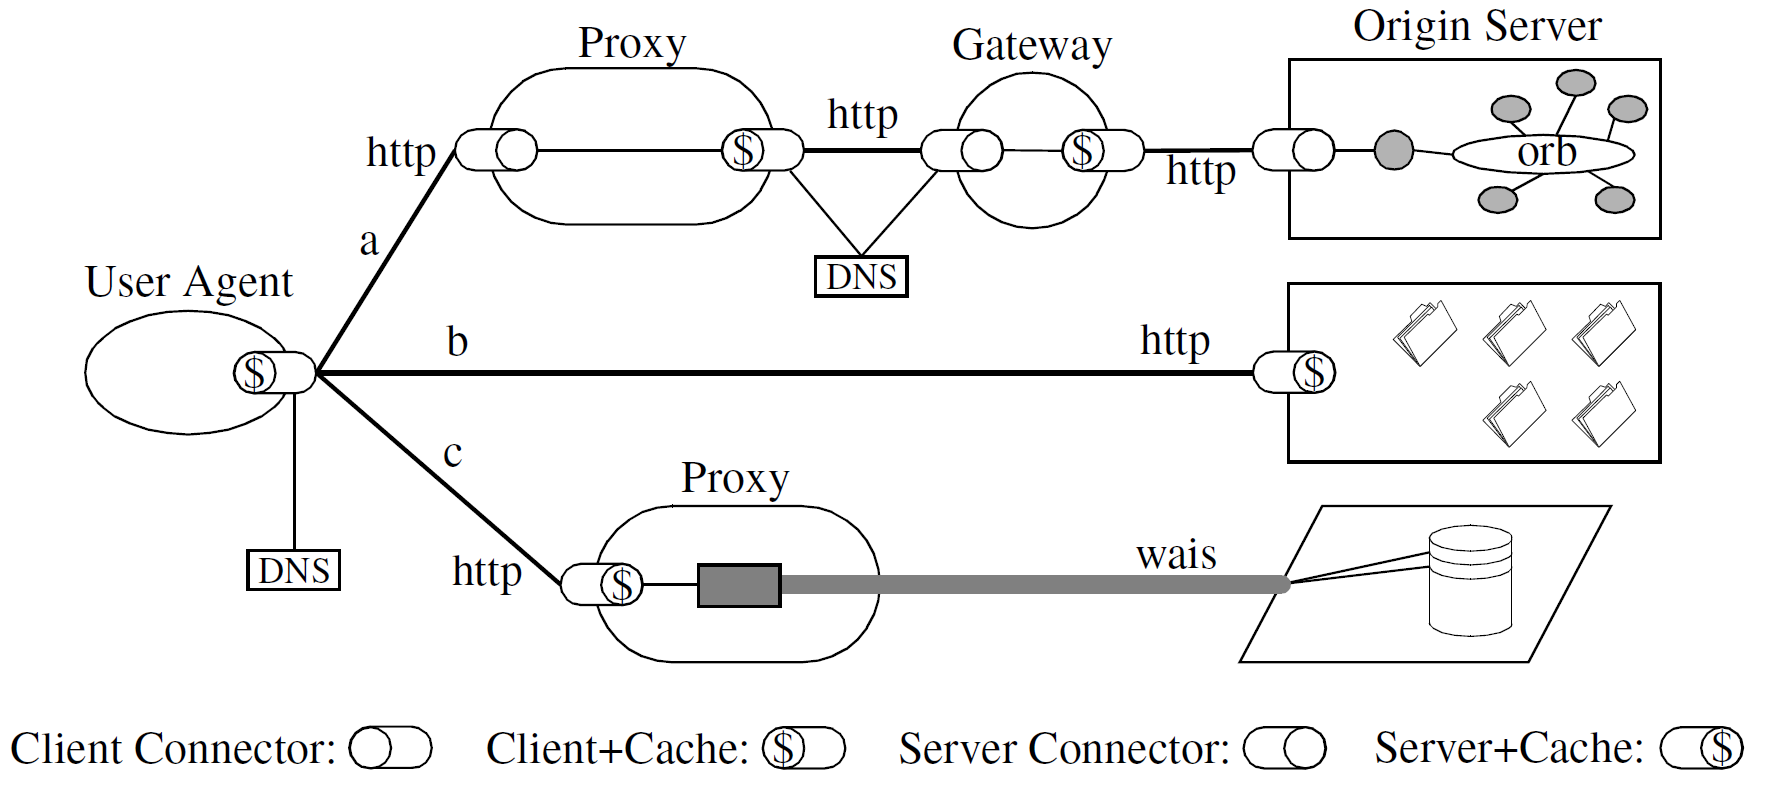
\includegraphics[width=\linewidth]{REST-process-view.png}
  \caption{REST~\cite[84]{REST}}\label{img:REST-diss}
\end{figure}

\section{Implementierung von RESTful APIs}
Die REST Architektur ist generell protokollunabhängig, durch die Arbeit von Fielding an HTTP und URI sind diese jedoch sehr geeignet für die Implementierung und waren auch das erste Anwendungsfeld.\cite[vgl.][109,116]{REST}
Eine API, die dem REST Architekturstil folgt, wird RESTful genannt.
Da die Dissertation von Fielding jedoch einige Implementierungsdetails schuldig bleibt bzw.\ bewusst \textcquote[86]{REST}{Details der Komponentenimplementierung und Protokollsyntax [ignoriert]}, wurde der Begriff RESTful API mit der Zeit aufgeweicht und für APIs verwendet, die grundlegende Anforderungen nicht erfüllen.\cite[vgl.][]{fieldBlog}
\par
\begin{itemize}
  \item Richardson Maturity Model ermöglicht Bestimmung wie REST konform Web service (API) ist
  \item Level 0
  \item Level 1
  URI
  \item Level 2
  \begin{itemize}
    \item HTTP Methoden genutzt als Kontrolldaten um Intention auszudrücken
    \item CRUD Operationen werden abgedeckt
    \item GET:\ Anfragen einer Repräsentation der Ressource
    \item POST:\ kann zum Erstellen, Modifizieren und Löschen von Ressourcen verwendet werden, schlecht definiert; Funktionsweise in folgende Methoden aufgeteilt
    \item PUT:\ Erstellen/Ersetzen einer Repräsentation
    \item PATCH:\ Modifizieren einer Repräsentation
    \item DELETE:\ Löschen der Ressource
    \item GET, PUT, DELETE sind idempotent (gleiches Ergebnis bei mehrmaliger Ausführung). GET ist safe (kein Verändern der Ressource).
  \end{itemize}
  \item Level 3
  \begin{itemize}
    \item Hypermedia ermöglicht Navigation durch die API\@. Client ändert seinen Zustand, indem er URIs (Links) folgt (HATEOAS)
    \item keine externe Dokumentation nötig. Links zwischen Dokumenten dokumentieren die Ressourcen
    \item Datenformat ist entscheidend. Bestimmte Formate haben native Unterstützung für Links und Forms (HTML, ATOM)
    \item Media Type bestimmt Auswertung (und Anzeige) der Antwort. JSON, XML können genutzt werden. Client benötigt Informationen über Datenstruktur, um Links in diesen Dokumenten auszuwerten.
  \end{itemize}
\end{itemize}

\section{Verbreitung und Standardisierung}
\begin{itemize}
  \item REST bestimmt nicht welches Format benutzt werden muss.
  \item Kein REST Standard
  \item REST APIs nutzen Web Standards (HTTP, URI, Hypermedia)
  \item XML und HTML zur direkten Anzeige geeignet. JSON beliebter geworden, das leichter für Menschen und Maschinen zu lesen
  \item verschiedene Ansätze um Struktur von JSON Dokumenten zur Verwendung in APIs zu definieren. Teilweise miteinander verwendbar (definieren verschiedene Aspekte der Kommunikation)
  \item OpenAPI
  \item JSON:API
  \item Abbildung Beispiel Request und Response
\end{itemize}
REST bleibt Implementierungsdetails schuldig\cite[vgl.][86]{REST}